\documentclass{beamer}
% for handouts: \documentclass[handout]{beamer}

%\setbeamertemplate{background canvas}[vertical shading][bottom=white,top=structure.fg!25]
% or whatever

\usetheme[compress]{Amsterdam}
%\setbeamertemplate{headline}{}
%\setbeamertemplate{footline}{}
%\setbeamersize{text margin left=0.5cm}
  
\usepackage[english]{babel}
\usepackage{listings}
\usepackage{geometry}
\usepackage{hyperref}

\usepackage{color}
\usepackage[T1]{fontenc}
\usepackage[utf8]{inputenc}
\usepackage{lmodern}

\lstset{
basicstyle=\scriptsize\ttfamily,
columns=flexible,
breaklines=true,
numbers=left,
%stepsize=1,
numberstyle=\tiny,
backgroundcolor=\color[rgb]{0.85,0.90,1}
}


\begin{document}

\title[Big Data and Automated Content Analysis]{\textbf{Big Data and Automated Content Analysis} \\ Week 3 -- Monday \\ \» Data harvesting and storage \«}
\author[Damian Trilling]{Anne Kroon \& Damian Trilling \\ ~ \\ \footnotesize{a.c.kroon@uva.nl \\ @annekroon \\ d.c.trilling@uva.nl \\@damian0604} \\ \url{www.damiantrilling.net}}
\date{19 February 2018}
\institute[UvA]{Afdeling Communicatiewetenschap \\Universiteit van Amsterdam}


\begin{frame}{}
\titlepage
\end{frame}

\begin{frame}{Today}
\tableofcontents
\end{frame}



\section{Last week's exercise}
\subsection{Step by step}
\begin{frame}[plain]
\textbf{Last week's exercise}\\
\vspace{1cm}
Discussing the code
\end{frame}



\begin{frame}[fragile]{Reading a JSON file into a dict, looping over the dict}
Task 1: Print all titles of all videos
\begin{lstlisting}
import json

with open("/home/damian/pornexercise/xhamster.json") as fi:
    data=json.load(fi)

for k,v in data.items()):
    print (v["title"])
            
\end{lstlisting}
\onslide<2->{
\footnotesize{NB: You have to know (e.g., by reading the documentation of the dataset) that the key is called \texttt{title}}}
\onslide<3->{\\
\footnotesize{NB: \texttt{data} is in fact a dict of dicts, such that each value \texttt{v} is another dict.\\ For each of these dicts, we retrieve the value that corresponds to the key \texttt{title}}}
\end{frame}


\begin{frame}[fragile]{What to do if you do not know the structure of the dataset?}
	Inspecting your data: use the functions \texttt{type()} and \texttt{len()} and/or the dictionary method \texttt{.keys()}
\begin{lstlisting}
len(data)
type(data)
data.keys()
	
\end{lstlisting}
	\onslide<2->{
		\footnotesize{\texttt{len()} returns the number of items of an object; \texttt{type()} returns the type object; \texttt{.keys()} returns a list of all available keys in the dictionary}}}
\end{frame}

\begin{frame}[fragile]{What to do if you do not know the structure of the dataset?}
	Inspecting your data: use the module \texttt{pprint} 
\begin{lstlisting}
from pprint import pprint

pprint(data)

\end{lstlisting}
\end{frame}


\begin{frame}[plain]{}
	\makebox[\linewidth]{
		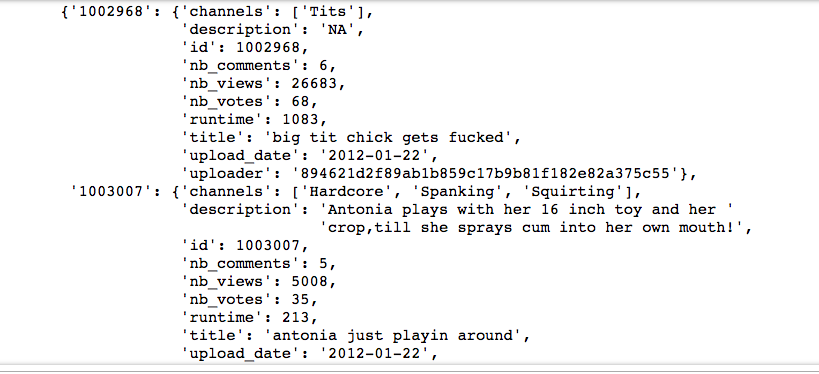
\includegraphics[width=\paperwidth,height=\paperheight,keepaspectratio]{../../pictures/pprint.png}
	}
\end{frame}

\begin{frame}[plain]{}
	\makebox[\linewidth]{
		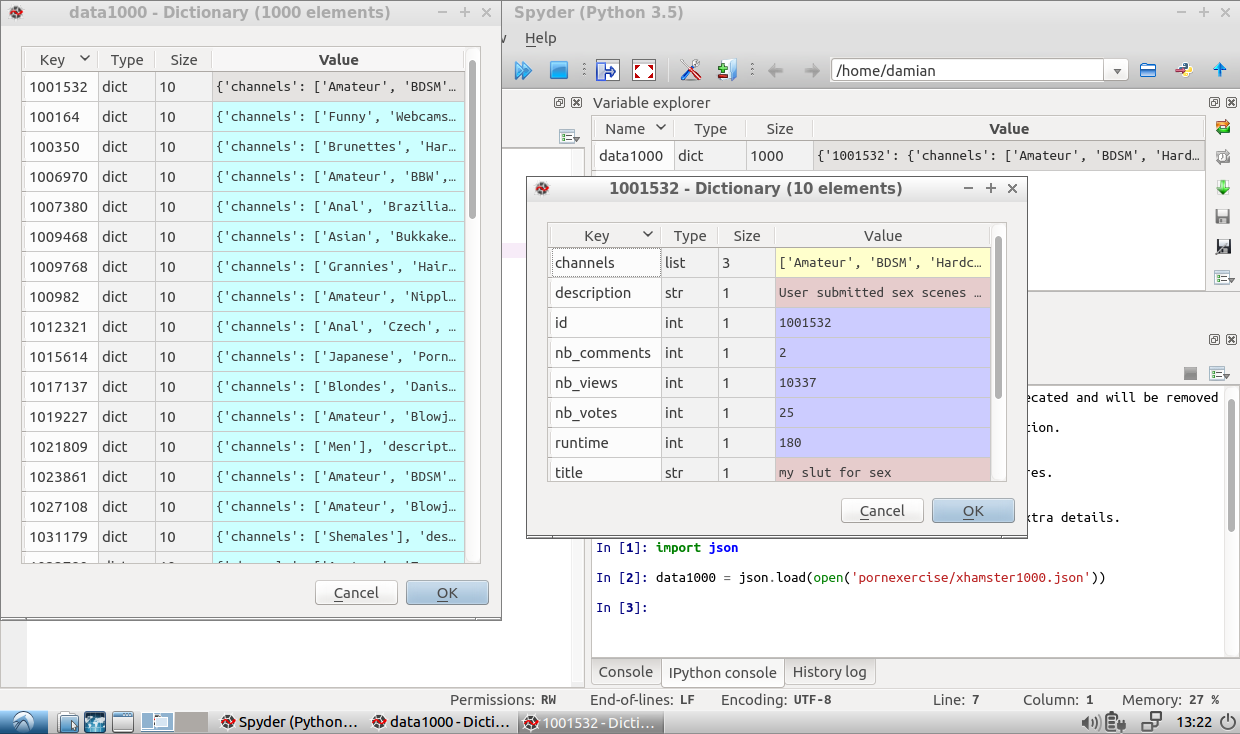
\includegraphics[width=\paperwidth,height=\paperheight,keepaspectratio]{../../pictures/spyder-dictofdicts.png}
	}
\end{frame}


\begin{frame}[fragile]{For the sake of completeness\ldots}
\texttt{.items()} returns a key-value \emph{pair}, that's why we need to assign \emph{two} variables in the for statement.

These alternatives would also work:
\begin{lstlisting}
for v in data.values()):
	print(v["title"])
\end{lstlisting}

\begin{lstlisting}
for k in data:      #or: for k in data.keys():
	print(data[k]["title"])
\end{lstlisting}

\textbf{Do you see (dis-)advantages?}
\end{frame}



\begin{frame}[fragile]{Working with a subset of the data}
	
What to do if you want to work with a smaller subset of the data?

Taking a random sample of 10 items in your dict:
	\begin{lstlisting}
import random
short_dict = dict(random.sample(data.items(),10))
	\end{lstlisting}
	
Taking the first 10 elements in a list:
	\begin{lstlisting}
short_list = list[:10]
	\end{lstlisting}

\end{frame}




\begin{frame}[fragile]{Initializing variables, merging two lists, using a counter}
Task 2: Average tags per video and most frequently used tags
\begin{lstlisting}
from collections import Counter
    
alltags=[]
i=0
for k,v in data.items():
    i+=1
    alltags+=v["channels"] # or: alltags.extend(v["channels"])

print(len(alltags),"tags are describing",i,"different videos")
print("Thus, we have an average of",len(alltags)/i,"tags per video")

c=Counter(alltags)
print (c.most_common(100))
\end{lstlisting}
\scriptsize{(there are other, more efficient ways of doing this)}

\end{frame}





\begin{frame}[fragile]{Nesting blocks, using a defaultdict to count, error handling}
Task 3: What porn category is most frequently commented on?
\begin{lstlisting}
from collections import defaultdict

commentspercat=defaultdict(int)
for k,v in data.items():
        for tag in v["channels"]:
            try:
                commentspercat[tag]+=int(v["nb_comments"])
            except:
                pass
print(commentspercat)
# if you want to print in a fancy way, you can do it like this:
for tag in sorted(commentspercat, key=commentspercat.get, reverse=True):
    print( tag,"\t", commentspercat[tag])
\end{lstlisting}
\scriptsize{A defaultdict is a normal dict, with the difference that the type of each value is pre-defined and it doesn't give an error if you look up a non-existing key}
\onslide<2->{\\~\\
\scriptsize{NB: In line 7, we assume the value to be an int, but the datasets sometimes contains the string ``NA'' instead of a string representing an int. That's why we need the try/except construction}}

\end{frame}



\begin{frame}[fragile]{Adding elements to a list, sum() and len()}
Task 4: Average length of descriptions
\begin{lstlisting}
length=[]
for k,v in data.items():
    length.append(len(v["description"]))
    
print ("Average length",sum(length)/len(length))
\end{lstlisting}

\end{frame}


\begin{frame}[fragile]{Merging vs appending}
Merging:
\begin{lstlisting}
l1 = [1,2,3]
l2 = [4,5,6]
l1 = l1 + l2
print(l1)
\end{lstlisting}
gives \texttt{[1,2,3,4,5,6]}
~\\

Appending:
\begin{lstlisting}
l1 = [1,2,3]
l2 = [4,5,6]
l1.append(l2)
print(l1)
\end{lstlisting}
gives \texttt{[1,2,3,[4,5,6]]}

\texttt{l2} is seen as \emph{one} element to append to \texttt{l1}
\end{frame}


\begin{frame}[fragile]{Tokenizing with .split()}
Task 5: Most frequently used words
\begin{lstlisting}
allwords=[]
for k,v in data.items():
    allwords+=v["description"].split()
c2=Counter(allwords)
print(c2.most_common(100))
\end{lstlisting}
\scriptsize{
\texttt{.split()} changes a string to a list of words.\\ \texttt{"This is cool''.split()} \\results in\\ \texttt{$[$"This", "is", "cool"$]$}\\
}
\end{frame}


\subsection{Concluding remarks}
\begin{frame}{Concluding remarks}
Make sure you fully understand the code!\\
\vspace{1cm}
Re-read the corresponding chapters\\
\vspace{1cm}
\textbf{PLAY AROUND!!!}\\
\end{frame}



\section{Data harvesting and storage}
\begin{frame}[plain]
\textbf{Data harvesting and storage}\\
\vspace{1cm}
An overview of APIs, scrapers, crawlers, RSS-feeds, and different file formats
\end{frame}



\subsection{APIs}
\begin{frame}
	Collecting data:\\
	APIs
\end{frame}



\begin{frame}{APIs}
	\makebox[\linewidth]{
		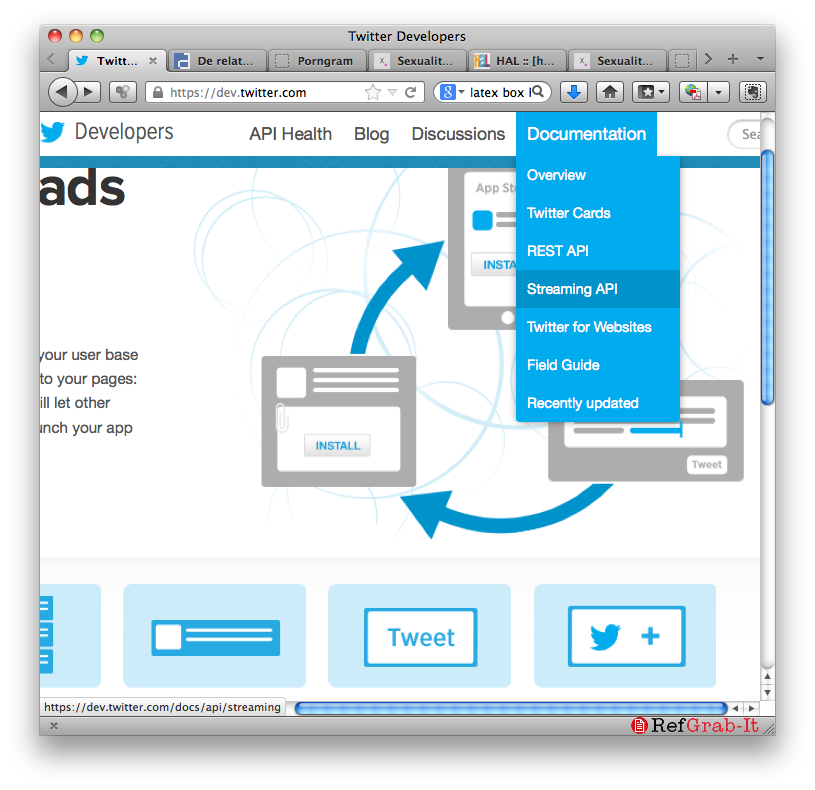
\includegraphics[width=\paperwidth,height=.8\paperheight,keepaspectratio]{../../pictures/dev_twitter_com.png}
	}
\end{frame}

\begin{frame}[fragile]{Querying an API}
	\begin{lstlisting}
# contact the Twitter API
auth = OAuth(access_key, access_secret, consumer_key, consumer_secret)
twitter = Twitter(auth = auth)
	
# get all info about the user 'username')
tweepinfo=twitter.users.show(screen_name=username)
	
# save his bio statement to the variable bio
bio=tweepinfo["description"])
	
# save his location to the variable location
location=tweepinfo["location"]	
\end{lstlisting}
	~\\ \tiny{(abbreviated Python example of how to query the Twitter REST API)}
\end{frame}


\begin{frame}{Who offers APIs?}
	The usual suspects: Twitter, Facebook, Google -- but also Reddit, Youtube, \ldots \\~
	\begin{block}{If you ever leave your bag on a bus on Chicago}<2->
		\onslide<3->{
			\ldots but do have Python on your laptop, watch this: \url{https://www.youtube.com/watch?v=RrPZza_vZ3w}. \\
			That guy queries the Chicago bus company's API to calculate when \emph{exactly the vehicle} with his bag arrives the next time at the bus stop in front of his office.
			\\~\\ \tiny{(Yes, he tried calling the help desk before, but they didn't know. He got his bag back.)}
		}
	\end{block}
\end{frame}

\begin{frame}{APIs}
	\begin{block}{Pro}<1->
		\begin{itemize}
			\item Structured data
			\item Easy to process automatically
			\item Can be directy embedded in your script
		\end{itemize}
	\end{block}
	\begin{block}{Con}<2->
		\begin{itemize}
			\item Often limitations (requests per minute, sampling, \ldots)
			\item You have to trust the provider that he delivers the right content {\footnotesize{($\Rightarrow$ Morstatter e.a., 2013)}}
			\item {\textbf{Some APIs won't allow you to go back in time!}}
		\end{itemize}
	\end{block}
	~\\
	\tiny{Morstatter, F., Pfeffer, J., Liu, H., \& Carley, K. M. (2013). Is the sample good enough? Comparing data from Twitter’s Streaming API with Twitter’s Firehose. \emph{International AAAI Conference on Weblogs and Social Media.} \\}
\end{frame}



%\subsection{APIs: Collecting tweets with DMI-TCAT}

\begin{frame}
	So we have learned that we can access an API directly. \\
	But what if we have to do so 24/7?
	\\~\\~\\
	\onslide<2->{Collecting tweets with a tool running on a server that \emph{does} query the API 24/7. \\~\\}
	
\end{frame}


\begin{frame}[t]{Data harvesting and storage}
	\begin{columns}
		\column{.3\textwidth}
		\makebox[\columnwidth]{
			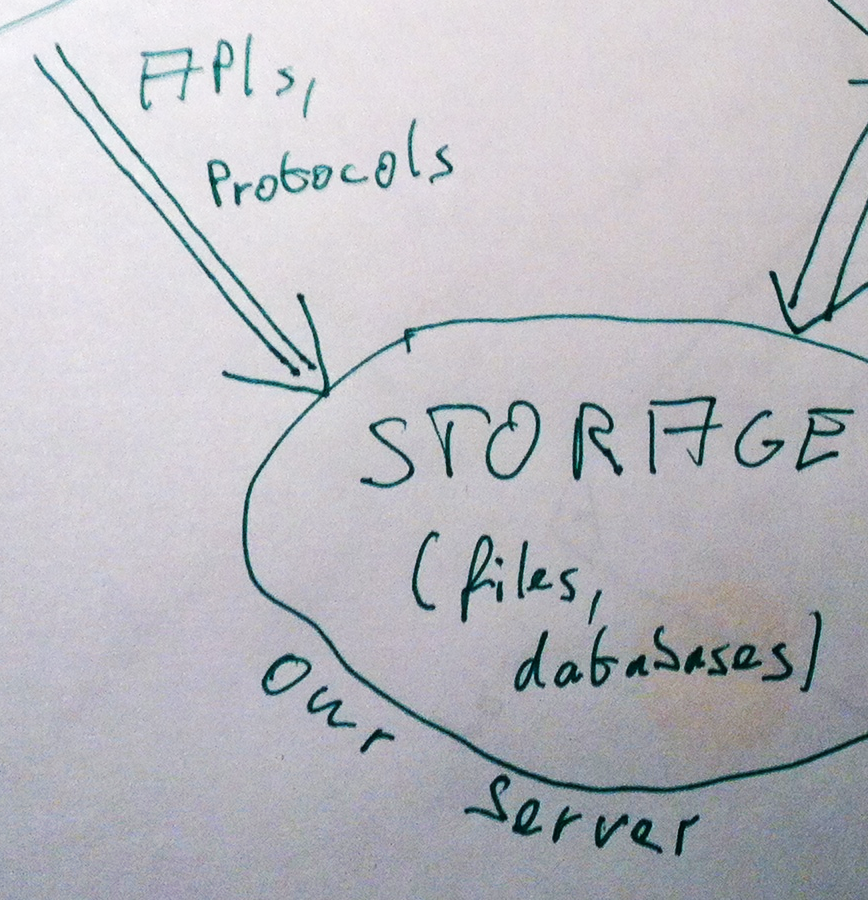
\includegraphics[width=\columnwidth,height=\paperheight,keepaspectratio]{../../pictures/process-storage.png}
		}
		\column{.7\textwidth}
		\begin{block}{It queries the API and stores the result}<2->
			It continuosly calls the Twitter-API and saves all tweets containing specific hashtags to a MySQL-database.
			\\~\\
			You tell it once which data to collect -- and wait some months.
		\end{block}
	\end{columns}
\end{frame}

\begin{frame}[t]{Data harvesting and storage}
	\begin{columns}
		\column{.3\textwidth}
		\makebox[\columnwidth]{
			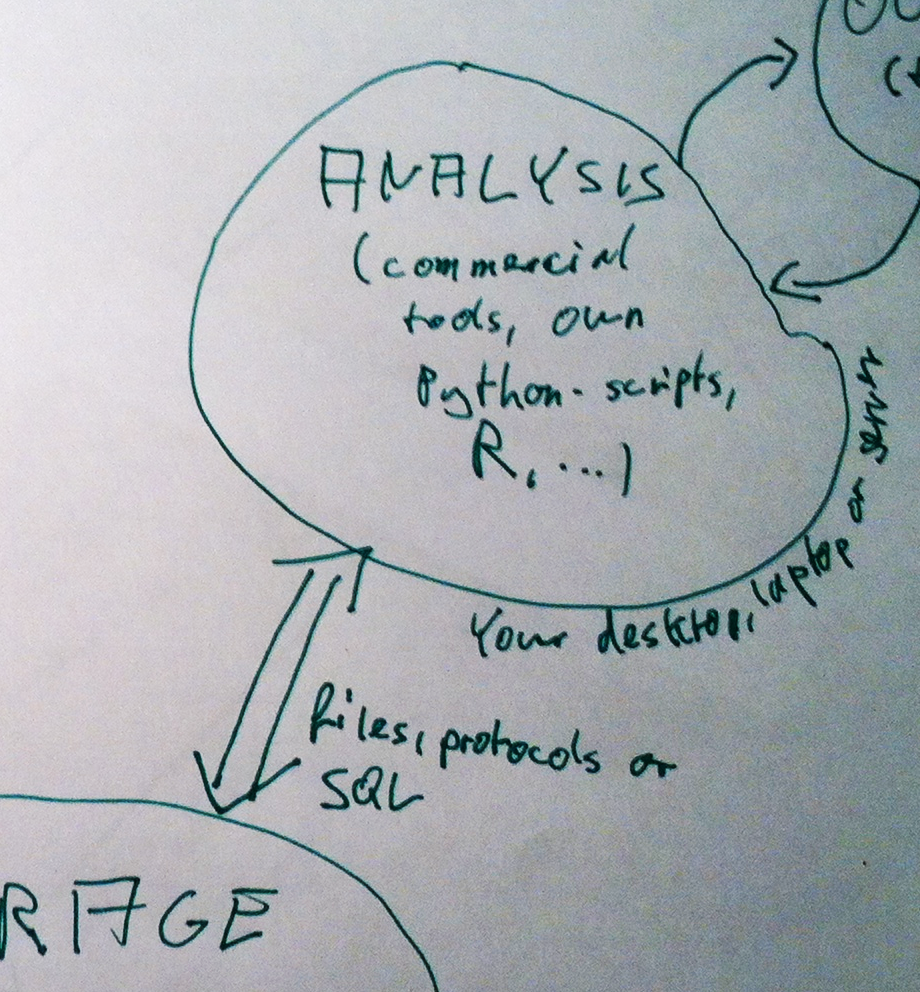
\includegraphics[width=\columnwidth,height=\paperheight,keepaspectratio]{../../pictures/process-analysis.png}
		}
		\column{.7\textwidth}
		\begin{block}{Retrieving the data for analysis}<2->
			You \emph{could} access the MySQL-database directly. 
			\\~\\
			Generally raw data needs to be cleaned and parsed, before you can start analyzing and visualizing
		\end{block}
	\end{columns}
\end{frame}


%{\setbeamercolor{background canvas}{bg=black}
%\begin{frame}[plain]
%\makebox[\linewidth]{
%\includegraphics[width=\paperwidth,height=\paperheight,keepaspectratio]{server_http-login.png}
%}
%\end{frame}
%}


\subsection{RSS feeds}
\begin{frame}
	Collecting data:\\
	RSS feeds
\end{frame}

\begin{frame}{RSS feeds}
	\begin{block}{What's that?}
		\begin{itemize}
			\item<1-> A structured (XML) format in which for example news sites and blogs offer their content
			\item<2-> You get only the new news items (and that's great!)
			\item<3-> Title, teaser (or full text), date and time, link
		\end{itemize}
	\end{block}
	\onslide<4->{
		\scriptsize{
			\url{http://www.nu.nl/rss} \\
			%\url{http://datacollection3.followthenews-uva.cloudlet.sara.nl/rsshond}\\
		}
	}
\end{frame}

\begin{frame}{RSS feed}
	\makebox[\linewidth]{
		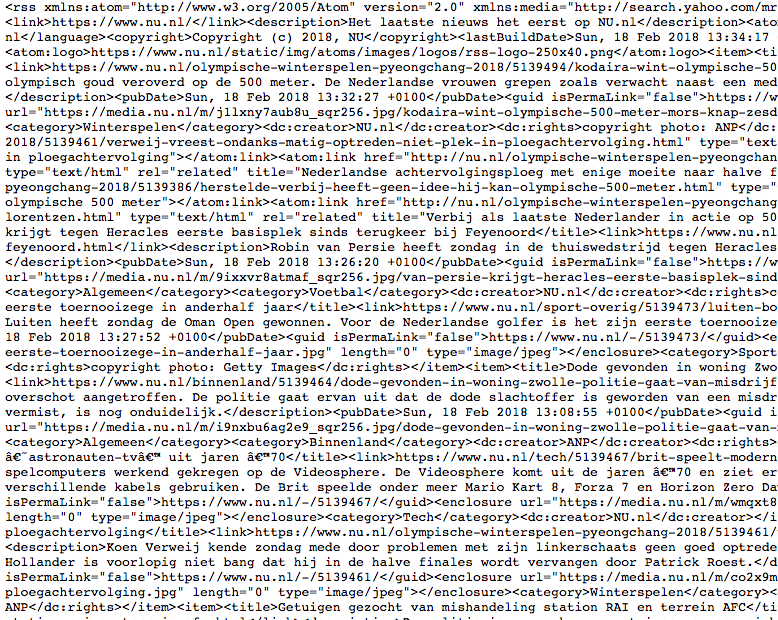
\includegraphics[width=\paperwidth,height=.8\paperheight,keepaspectratio]{../../pictures/rss_nl.png}
	}
\end{frame}


\begin{frame}[fragile]{Parsing RSS feeds}
\begin{lstlisting}
	
tree = fromstring(htmlsource)
	
# parsing article teaser
try:
    teaser=tree.xpath('//*[@class="item-excerpt"]//text()')[0]
except:
    logger.debug("Could not parse article teaser.")
    teaser=""
	
# parsing article text
try:
    text=" ".join(tree.xpath('//*[@class="block-wrapper"]/div[@class="block-content"]/p//text()')).strip()
except:
    text = ""
    logger.warning("Could not parse article text")
	
\end{lstlisting}
~\\ \tiny{(abbreviated Python example of how to parse the RSS feed of NU.nl)}
\end{frame}


\begin{frame}{RSS feeds}
\begin{block}{Pro}
\begin{itemize}
\item \emph{One} protocol for all services
\item Easy to use
\end{itemize}
\end{block}

\begin{block}{Con}
\begin{itemize}
\item Full text often not included, you have to download the link separately ($\Rightarrow$ Problems associated with scraping) 
\item {\textbf{You can't go back in time!}} \footnotesize{But we have archived a lot of RSS feeds}
\end{itemize}
\end{block}

\end{frame}

\subsection{Scraping and crawling}
\begin{frame}
Collecting data:\\
Scraping and crawling
\end{frame}

\begin{frame}{Scraping and crawling}
\begin{block}{If you have no chance of getting already structured data via one of the approaches above}
\begin{itemize}
\item<2->Download web pages, try to identify the structure yourself
\item<2->You have to \emph{parse} the data
\item<3-> Can get very complicated (depending on the specific task), especially if the structure of the web pages changes
\end{itemize}
\end{block}
\onslide<3->{
{\scriptsize{Further reading:\\
\url{http://scrapy.org}\\
\url{ https://github.com/anthonydb/python-get-started/blob/master/5-web-scraping.py} \\
}}}
\end{frame}

		
\subsection{Parsing text files}
\begin{frame}
Collecting data:\\
Parsing text files
\end{frame}

\begin{frame}{For messy input data or for semi-structured data}
Guiding question: Can we identify some kind of pattern?
\begin{block}{Examples}<2->
\begin{itemize}
\item<2-> Lewis, Zamith, \& Hermida (2013) had a corrupt CSV-file
\item<3-> LexisNexis gives you a chunk of text (rather than, e.g., a structured JSON or XML object)
\end{itemize}
\onslide<4->{But in both cases, as long as you can find any pattern or structure in it, you can try to write a Python script to \emph{parse} the data.}
\end{block}
~\\

\onslide<2>{\tiny{Lewis, S. C., Zamith, R., \& Hermida, A. (2013). Content analysis in an era of Big Data: A hybrid approach to computational and manual methods. \emph{Journal of Broadcasting \& Electronic Media, 57}(1), 34–52. doi:10.1080/08838151.2012.761702\\}}
\end{frame}

{\setbeamercolor{background canvas}{bg=black}
\begin{frame}[plain]
\makebox[\linewidth]{
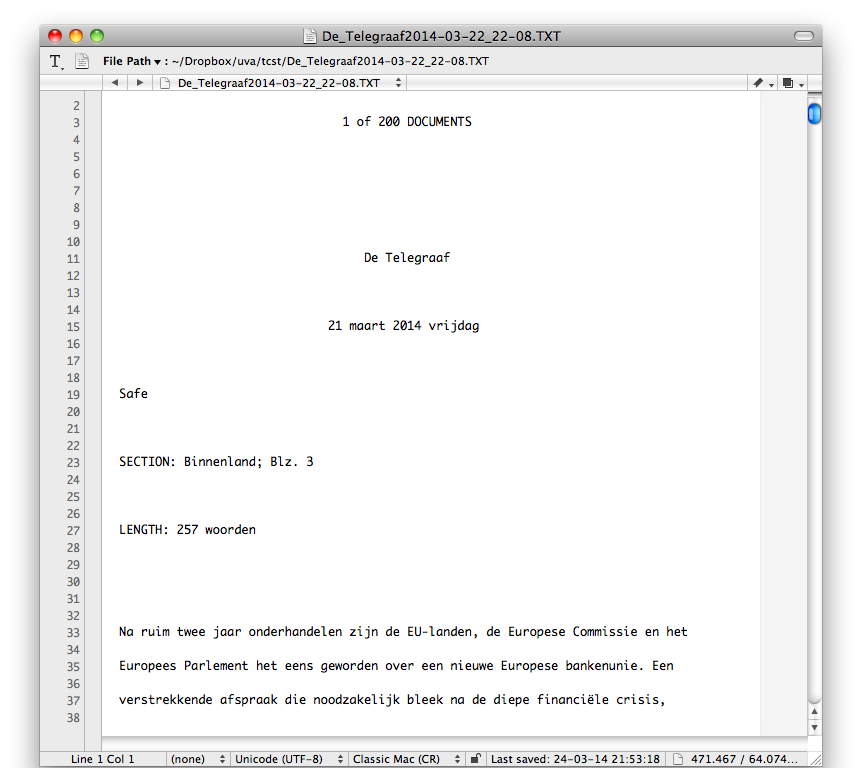
\includegraphics[width=\paperwidth,height=\paperheight,keepaspectratio]{../../pictures/lexisnexistxt.png}
}
\end{frame}
\begin{frame}[plain]
\makebox[\linewidth]{
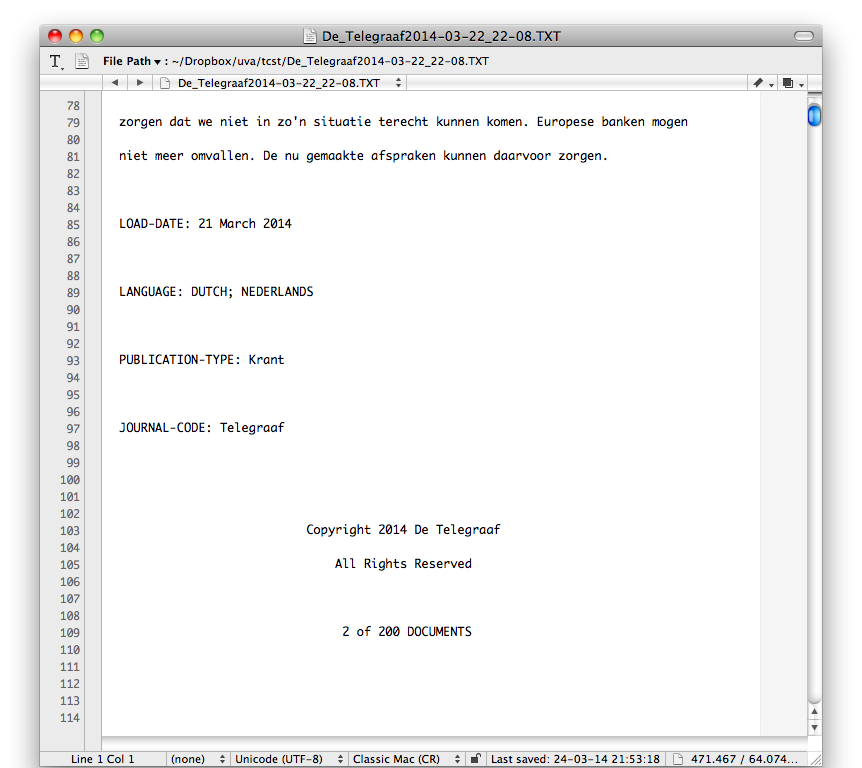
\includegraphics[width=\paperwidth,height=\paperheight,keepaspectratio]{../../pictures/lexisnexistxt2.png}
}
\end{frame}



\begin{frame}[plain,fragile]
\begin{lstlisting}
tekst={}
section={}
length={}
...
...
with open(bestandsnaam) as f:
  for line in f:
    line=line.replace("\r","")
    if line=="\n":
      continue
    matchObj=re.match(r"\s+(\d+) of (\d+) DOCUMENTS",line)
    if matchObj:
      artikelnr= int(matchObj.group(1))
      tekst[artikelnr]=""
      continue
    if line.startswith("SECTION"):
      section[artikelnr]=line.replace("SECTION: ","").rstrip("\n")
    elif line.startswith("LENGTH"):
      length[artikelnr]=line.replace("LENGTH: ","").rstrip("\n")
...
...
...

    else:
      tekst[artikelnr]=tekst[artikelnr]+line
\end{lstlisting}
\end{frame}

\end{frame}


\section{Storing data}

\subsection{CSV tables}
\begin{frame}
Storing data:\\
CSV tables
\end{frame}

\begin{frame}{CSV-files}
\begin{block}{Always a good choice}
\begin{itemize}
\item \emph{All} programs can read it
\item Even human-readable in a simple text editor:
\item Plain text, with a comma (or a semicolon) denoting column breaks
\item No limits regarging the size
\item But: several dialects (e.g., \texttt{,} vs. \texttt{;} as delimiter)
\end{itemize}
\end{block}
\end{frame}


\begin{frame}[fragile]{A CSV-file with tweets}
\begin{lstlisting}
text,to_user_id,from_user,id,from_user_id,iso_language_code,source,profile_image_url,geo_type,geo_coordinates_0,geo_coordinates_1,created_at,time
:-) #Lectrr #wereldleiders #uitspraken #Wikileaks #klimaattop http://t.co/Udjpk48EIB,,henklbr,407085917011079169,118374840,nl,web,http://pbs.twimg.com/profile_images/378800000673845195/b47785b1595e6a1c63b93e463f3d0ccc_normal.jpeg,,0,0,Sun Dec 01 09:57:00 +0000 2013,1385891820
Wat zijn de resulaten vd #klimaattop in #Warschau waard? @EP_Environment ontmoet voorzitter klimaattop @MarcinKorolec http://t.co/4Lmiaopf60,,Europarl_NL,406058792573730816,37623918,en,<a href="http://www.hootsuite.com" rel="nofollow">HootSuite</a>,http://pbs.twimg.com/profile_images/2943831271/b6631b23a86502fae808ca3efde23d0d_normal.png,,0,0,Thu Nov 28 13:55:35 +0000 2013,1385646935\end{lstlisting}
\end{frame}



\subsection{JSON and XML}
\begin{frame}
Storing data:\\
JSON and XML
\end{frame}

\begin{frame}{JSON and XML}
\begin{block}{Great if we have a nested data structure}
\begin{itemize}
\item<2-> Items within feeds
\item<3-> Personal data within authors within books
\item<4-> Tweets within followers within users
\end{itemize}
\end{block}
\end{frame}


\begin{frame}[fragile]{A JSON object containing GoogleBooks data}
\begin{lstlisting}
{'totalItems': 574, 'items': [{'kind': 'books#volume', 'volumeInfo': {'publisher': '"O\'Reilly Media, Inc."', 'description': u'Get a comprehensive, in-depth introduction to the core Python language with this hands-on book. Based on author Mark Lutz\u2019s popular training course, this updated fifth edition will help you quickly write efficient, high-quality code with Python. It\u2019s an ideal way to begin, whether you\u2019re new to programming or a professional developer versed in other languages. Complete with quizzes, exercises, and helpful illustrations, this easy-to-follow, self-paced tutorial gets you started with both Python 2.7 and 3.3\u2014 the
...
...
'kind': 'books#volumes'}
\end{lstlisting}
\end{frame}

\begin{frame}[fragile]{An  XML object containing an RSS feed}
\begin{lstlisting}
...
<item>
        <title>Agema doet aangifte tegen Samsom en Spekman</title>
        <link>http://www.nu.nl/politiek/3743441/agema-doet-aangifte-samsom-en-spekman.html</link>
         <guid>http://www.nu.nl/politiek/3743441/index.html</guid>
         <description>PVV-Kamerlid Fleur Agema gaat vrijdag aangifte doen tegen PvdA-leider Diederik Samsom en PvdA-voorzitter Hans Spekman wegens uitspraken die zij hebben gedaan over Marokkanen. </description>
         <pubDate>Thu, 03 Apr 2014 21:58:48 +0200</pubDate>
        <category>Algemeen</category>
         <enclosure url="http://bin.snmmd.nl/m/m1mxwpka6nn2_sqr256.jpg" type="image/jpeg" />
         <copyrightPhoto>nu.nl</copyrightPhoto>        
</item>
...
\end{lstlisting}
\end{frame}



\begin{frame}{It's the same as our ``dict of dicts''/``dict of lists''/\ldots data model!}
	\makebox[\linewidth]{
		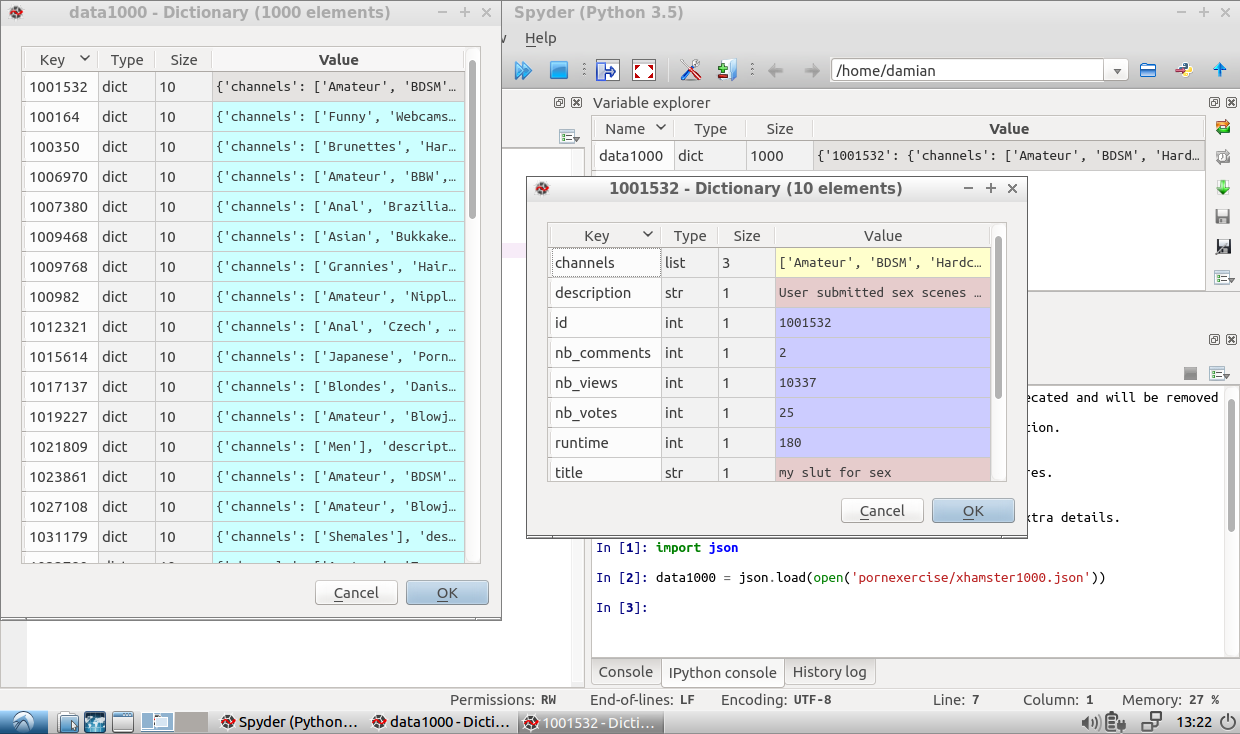
\includegraphics[width=\paperwidth,height=.8\paperheight,keepaspectratio]{../../pictures/spyder-dictofdicts.png}
	}
\end{frame}		
		
		
\section{Next meetings}
\begin{frame}
Next meetings
\end{frame}

\begin{frame}{Next meetings}
\begin{block}{Wednesday, 21--3}
Writing some first data collection scripts
\end{block}
	
\end{frame}




\end{document}

